查看本节演示代码：\demonotebook{05}{5.6_Data-reuploading_classifier} \ \demonotebookgithub{05}{5.6_Data-reuploading_classifier}

\subsubsection{背景}

% Run-Hong He, State Key Laboratory of Computer Science, Institute of Software Chinese Academy of Science, BeiJing 101408, China

数据分类不仅是经典神经网络的重要应用，也是量子信息与量子计算未来的重要应用方向。量子分类器的结构通常可以分为三个主要部分：负责数据编码的子线路、用于信息处理的子线路，以及为了从末态中提取分类结果而执行的测量。
实现高精度数据分类的关键在于捕获数据的非线性特征。许多方法都会精心设计量子线路以引入这种能力，例如受人工神经网络启发的策略，或经典机器学习中广泛使用的核方法 \cite{PhysRevLett.122.040504, 2019Supervised_nature, Wan_2017_npjqi, hur2022quantum, chalumuri2021hybrid, oh2020tutorial, farhi2018classification, wrobel2021application}。在当前 NISQ 设备阶段，需要更少资源（如量子比特数和量子操作数）的方案受到了广泛关注。
因此，一个自然的研究动机是探索构造有效量子分类器所需的最小资源。

文献 \cite{PerezSalinas2020datareuploading} 表明，借助一个经典子程序，单个量子比特就可以提供足够的计算能力，对多维输入数据执行多分类任务，其作用类似于单隐藏层神经网络。这个结论或许令人意外，尤其是考虑到单个量子比特只提供两个样本态的叠加，而作用在其上的操作本质上只是 Bloch 球上的旋转。
该方案的核心在于把数据上传单元和信息处理单元结合起来，并多次重复这一结构，即采用\textit{数据重上传}（Data re-uploading）机制，为监督分类任务引入必要的非线性。

\begin{figure}
	\centering
	\begin{subfigure}{0.3\textwidth}
		\centering
		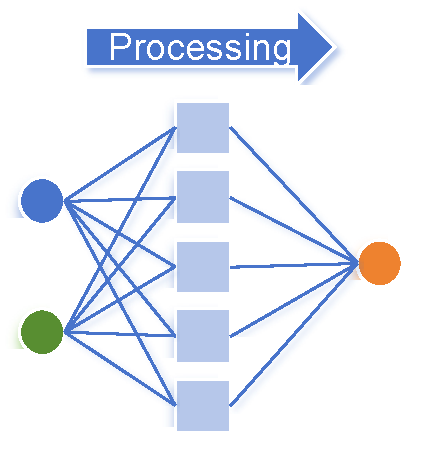
\includegraphics[width=\textwidth]{5.4.3_figures/data_reuploading_neural_network.pdf}
		\caption{经典神经网络。}
	\end{subfigure}
	\begin{subfigure}{0.3\textwidth}
		\centering
		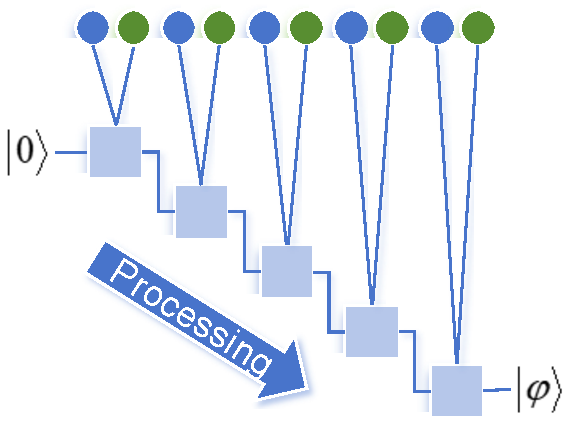
\includegraphics[width=0.9\textwidth]{5.4.3_figures/data_reuploading_quantum_classifier.pdf}
		\caption{量子分类器。}
	\end{subfigure}
    \captionsetup{justification=raggedright,singlelinecheck=false}
    \caption{（a）单隐藏层经典神经网络与（b）具有数据重上传结构的单量子比特量子分类器的简化工作流程。
    在经典神经网络中，每个神经元都会接收全部输入数据。相应地，量子比特既接收输入数据，也接收前序操作的结果；它对组合后的信息进行处理，最终输出一个量子态，其中编码了多次输入上传和处理参数。}
    \label{diagram_data_reuploading}
\end{figure}

作者在工作中证明，数据重上传方案与著名的通用逼近定理 \cite{HORNIK1991251} 具有等价关系；该定理指出，由足够多神经元和激活单元组成的单层网络可以逼近任意连续函数。

在构造单量子比特分类器之前，我们先从经典单层神经网络的工作流程入手。
如图 \ref{diagram_data_reuploading}（a）所示，原始数据被输入并由每个神经元处理；换言之，原始数据被多次重新上传。随后，结合激活函数，这个前馈神经网络便能够捕获非线性。

为了把这种能力引入单量子比特分类器，我们同样需要在不违背量子不可克隆定理的前提下，反复把数据上传到量子比特中。数据重上传方案 \cite{PerezSalinas2020datareuploading} 正是为解决这一问题而设计，其工作流程如图 \ref{diagram_data_reuploading}（b）所示。与经典神经网络类似，数据点会同时进入单量子比特量子分类器中的每个处理单元；这里的处理单元由一个酉旋转表示。
不过，处理单元不仅受输入数据影响，也受之前处理单元的影响。
最终输出是一个量子态，需要通过测量来提取分类结果。

\begin{figure}[h]
    \begin{center}
        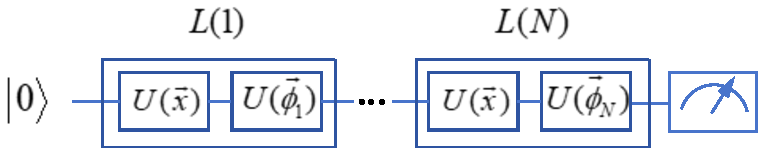
\includegraphics[width=0.9\linewidth]{5.4.3_figures/data_reuploading_circuit.pdf}
    \end{center}
    \captionsetup{justification=raggedright,singlelinecheck=false}
    \caption{带数据重上传的单量子比特分类器由若干层 $L(i)$ 组成，这些层构成量子线路的基本模块。每一层包含负责数据上传的 $U(x)$ 门，以及一个可训练的参数化酉变换 $U(\phi)$。该基本模块重复 $N$ 次后，计算一个代价函数；该函数与线路末态和对应类别目标态之间的保真度相关。}
    \label{data_reuploading_circuit}
\end{figure}

该单量子比特分类器的显式形式如图 \ref{data_reuploading_circuit} 所示。经典数据按顺序被反复重上传，相邻的数据上传单元之间插入处理单元。引入的数据可以表示为量子比特旋转。对于三维空间中的数据点 $\overrightarrow{x}$，可以通过量子比特旋转 $U(\overrightarrow{x})$ 进行重上传。后续处理单元同样是旋转，其旋转角作为可训练参数优化，以最小化代价值 $C(F)$ 并提升性能。保真度 $F$ 用于量化线路末态与标签对应目标态之间的接近程度。

于是，该量子线路的整体函数为
$$\mathcal{U}(\overrightarrow{\phi},\overrightarrow{x})=U(\overrightarrow{\phi}_N)U(\overrightarrow{x})\cdots U(\overrightarrow{\phi}_1)U(\overrightarrow{x}),$$
其作用为
$$|\varphi\rangle=\mathcal{U}(\overrightarrow{\phi},\overrightarrow{x})|0\rangle.$$
数据点的最终类别将由对 $|\phi\rangle$ 的测量结果决定。每一对数据上传单元和处理单元可以共同组成一个处理层：
$$L(i)\equiv U(\overrightarrow{\phi}_i)U(\overrightarrow{x}),$$
因此分类器可写为
$$\mathcal{U}(\overrightarrow{\phi},\overrightarrow{x})=L(N)\cdots L(1).$$

作者指出，增加层数可以赋予线路更强的表达能力，从而带来更高的分类精度。

\textbf{目标问题：}

构造并训练一个单量子比特数据重上传量子线路，用于对经典数据进行分类。

\textbf{所需的 MindSpore Quantum 功能：}

1. 支持构造交错且重复的 encoder 与 ansatz 线路，并允许向 encoder 进行数据重上传。

2. 支持对输入数据（多组数据和标签）进行批量训练。

\subsubsection{实现}

在本示例中，我们关注一个典型的分类任务：识别平面上不同区域内的点，并基于 \MindQuantum\ 实现该任务。

我们创建一个数据集，其中包含大量坐标为 $\overrightarrow{x}=(x_1, x_2)$、随机分布在单位面积平面（$x\in[-1,1]$）上的点。
分类器的任务是根据这些数据点的坐标，判断其是否落在半径为 $r$ 的圆内，即是否满足 $x_1^2+x_2^2<r^2$。
这里特意将圆的半径设为 $r=\sqrt{\frac{2}{\pi}}$，以保证点位于圆内（标签为 ``0''，对应目标量子态 $|0\rangle$）和圆外（标签为 ``1''，对应目标量子态 $|1\rangle$）的概率相等。

\begin{lstlisting}
import numpy as np

def data_gen(n_samples=1000):
    center=[0.0, 0.0]
    rad=np.sqrt(2/np.pi)
    data, labels = [], []
    for i in range(n_samples):
        x = 2*(np.random.rand(2))-1
        if np.linalg.norm(x-center) <= rad:
            y = 0
        else:
            y = 1
        data.append(x)
        labels.append(y)
    return np.array(data), np.array(labels)

train_data, train_labels = data_gen(1000)
eval_data, eval_labels = data_gen(500)
test_data, test_labels = data_gen(5000)
\end{lstlisting}

我们创建的训练集、验证集和测试集分别包含 1000、500 和 5000 个随机样本。

为了把数据编码到量子比特上，我们使用围绕 $x$ 轴和 $z$ 轴旋转的角度来表示样本的坐标信息，即 $U(\overrightarrow{x})=U(x_1,x_2,0)=RZ(x_2)RX(x_1)$。由于待分类样本只有二维，这里补入了一个 0。
对于 $N$ 维输入数据（$[x_1, x_2, x_3, \cdots x_{N-2}, x_{N-1},x_{N}]$），可以将其划分为多组三维分量进行编码，即 $U(\overrightarrow{x})=U(x_{N-2},x_{N-1},x_{N})\cdots U(x_1,x_2,x_3)$。

接下来构造单量子比特分类器的线路。我们首先在初始量子态上作用 $H$ 门，以生成叠加态 $(|0\rangle+|1\rangle)/\sqrt{2}$。
随后加入 $RZ(x_1)$ 和 $RX(x_2)$ 门，把样本坐标 $x_1$ 和 $x_2$ 上传到量子比特上。
后续处理单元由带有三个独立可训练参数的 $U3$ 门表示，用以实现任意旋转。
这两个子线路也分别称为 ``encoder'' 和 ``ansatz''，以表明旋转门中的参数是直接输入的，还是在训练过程中逐步更新的。
encoder 与 ansatz 共同组成一层，重复多层即可实现多次数据重上传和处理，从而完成点分类。

\begin{lstlisting}

from mindquantum import H, RZ, RX, U3, BarrierGate, Circuit, Simulator, Hamiltonian, QubitOperator, MQLayer

def circ(depth=1):
    circ = Circuit(H.on(0))
    circ += BarrierGate()
    for layer in range(depth):
        circ += Circuit([RZ('x1').on(0), RX('x2').on(0)]).as_encoder()
        circ += Circuit(U3(f'theta_{layer}', f'phi_{layer}',f'lambda_{layer}').on(0)).as_ansatz()
        circ += BarrierGate()
    return circ

example_circ = circ(depth=1)
example_circ.svg()
\end{lstlisting}

\begin{figure}[H]
\centering
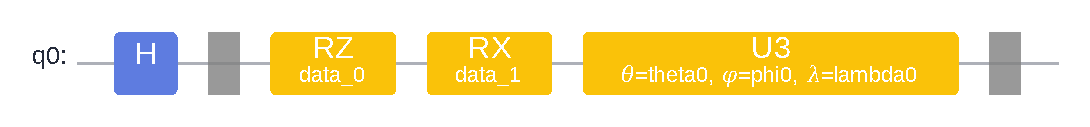
\includegraphics[width=0.49\textwidth]
{5.4.3_figures/data_reuploading_circ0.pdf}
\caption{示意图展示了单个量子比特先经过 $H$ 门生成均匀叠加态，随后通过一个编码层和信息处理层来处理分类任务。}
\label{data_reuploading_circ0}
\end{figure}

整体量子线路会把量子态从 $|0\rangle$ 变换为 $|\varphi\rangle$，随后需要对其进行测量。
如前所述，可以根据单量子比特的最终测量结果判断分类结果 ``0''（圆内）或 ``1''（圆外）；例如，当输出概率满足 $P(|0\rangle)>P(|1\rangle)$ 时，可将采样点分类为 ``0''，否则分类为 ``1''。
这一方法也可以用末态沿 $Z$ 方向的能量期望来表示：若 $E(|\varphi\rangle)>0$，则将采样点分类为 ``0''，否则分类为 ``1''。因此，损失函数可定义为 $Loss=[E(|\varphi\rangle)-(1-2\cdot\mathrm{label})]^2$。

在下面的代码中，我们使用学习率为 0.02 的 Adam 优化器作为经典子程序，训练量子线路中的可训练参数。通过最小化损失函数，分类性能将逐步提升。

\begin{lstlisting}
import mindspore as ms
from mindspore import Tensor, ops
from mindspore.nn import Adam, TrainOneStepCell, LossBase,WithLossCell
ms.set_context(mode=ms.PYNATIVE_MODE, device_target='CPU')
import copy

circ = circ(depth=4)
ham = Hamiltonian(QubitOperator('Z0'))
sim = Simulator('mqvector', 1)
grad_ops = sim.get_expectation_with_grad(ham, circ)
qnet = MQLayer(grad_ops)

class MyLoss(LossBase):
    def __init__(self, reduction='mean'):
        super(MyLoss, self).__init__(reduction)
        self.square = ops.Square()

    def construct(self, logits, label):
        out =self.square(logits - (1-2*label))
        return self.get_loss(out)

loss = MyLoss()
opti = Adam(qnet.trainable_params(), learning_rate=0.02)
model = TrainOneStepCell(WithLossCell(qnet, loss), opti)

\end{lstlisting}
如果需要用这个单量子比特分类器处理多类别任务，一种可行策略是将概率 $P(|0\rangle)$ 与多个阈值进行比较。例如，对于四分类任务，可以根据概率 $P(|0\rangle)$ 所在的区间来确定分类结果，其中 $0\leqslant\lambda_1\leqslant\lambda_2\leqslant\lambda_3\leqslant1$。

接下来，我们对 ansatz 中的参数训练 5000 次迭代，记录并保存训练过程中达到的最高验证精度及对应的可训练参数。训练批大小为 4。

\begin{lstlisting}
def eval(ansatz_params, eval_data, eval_labels):
    res = []
    for index in range(len(eval_label)):
        sim.reset()
        sim.apply_circuit(circ, pr=dict(zip(circ.params_name, np.hstack((eval_data[index], ansatz_params)))))
        exp = sim.get_expectation(ham).real
        clas = exp <= 0
        res.append(int(clas == eval_label[index]))
    return np.sum(res)/len(res)

acc_list = []
acc_max = 0.0

print('Training begins ...')

for i in range(2001):
    index = np.random.randint(0,len(train_data),4)
    loss = model(ms.Tensor(train_data[index]), ms.Tensor(train_labels[index]))
    acc = eval(qnet.weight.asnumpy(), eval_data, eval_labels)
    if acc > acc_max:
        acc_max = acc
        best_params = copy.deepcopy(qnet.weight.asnumpy())
    acc_list.append(acc)
    if i % 200 == 0:
        print(f'turn:{i}\t',f'\tacc_max:{acc_max}')

print('Training completes.\n')
print('Maximum validation accuracy in training:\n', acc_max)

test_acc = eval(best_params,test_data,test_labels)

print('Average test accuracy:\n', test_acc)
\end{lstlisting}

\begin{lstlisting}
Training begins ...
turn:0	 	  acc_max:0.55
turn:200	 	acc_max:0.566
turn:400	 	acc_max:0.622
turn:600	 	acc_max:0.622
turn:800	 	acc_max:0.7
turn:1000	 	acc_max:0.814
turn:1200	 	acc_max:0.814
turn:1400	 	acc_max:0.814
turn:1600	 	acc_max:0.814
turn:1800	 	acc_max:0.894
turn:2000	 	acc_max:0.894
Training completes.

Maximum validation accuracy in training:
0.894

Average test accuracy:
0.8876
\end{lstlisting}

从上述打印信息可以看出，模型预测精度已经达到 $88.76\%$，说明预期分类结果与实际分类结果吻合良好。
图 \ref{data_reuploading_performance} 对训练前的预测结果、训练后的预测结果和真实分类数据进行了可视化比较。
可以看到，经过训练后，这个单量子比特分类器能够有效区分样本。
\begin{figure}[H]
\centering
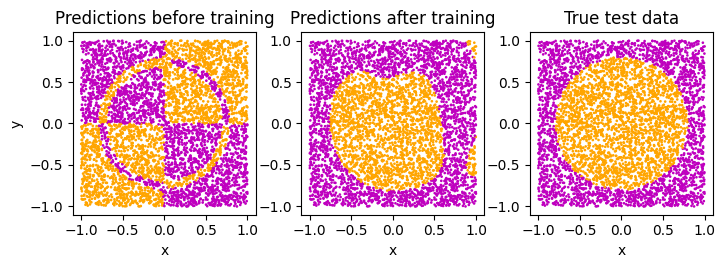
\includegraphics[width=0.49\textwidth]
{5.4.3_figures/data_reuploading_performance.png}
\caption{数据重上传单量子比特分类器在训练前、训练后以及真实数据上的预测结果可视化比较。}
\label{data_reuploading_performance}
\end{figure}

此外，作者还将该方案扩展到多量子比特版本。受益于更复杂的量子叠加态和量子纠缠，多量子比特方案取得了进一步提升的性能。
